\documentclass{beamer}
\usetheme{default}
\setbeamertemplate{navigation symbols}{\insertframenumber}%remove navigation symbols, but keep slide numbers
  
  \usepackage{tikz}
\usepackage{amsmath}
\usepackage{rotating}
\usepackage{ulem}
\usepackage{graphicx}
\usepackage{animate}
\usepackage{url}

\definecolor{darkgreen}{RGB}{0,200,0}
\definecolor{brickred}{RGB}{200,0,0}
\definecolor{darkblue}{RGB}{0,0,200}
\setbeamercolor{block title}{use=structure,fg=darkblue,bg=blue!7!white}
\setbeamercolor{block body}{use=structure,fg=black,bg=blue!7!white}

\DeclareMathOperator{\grad}{grad}
\DeclareMathOperator{\retr}{retr}
\DeclareMathOperator{\im}{im}

\usepackage[noend]{algorithmic}

\usepackage{tikz-cd}
\usetikzlibrary{cd}

\begin{document}


\title{Graph neural networks and graph isomorphism}
\author{Soledad Villar}
\institute{Center for Data Science\\Courant Institute of Mathematical Sciences \\ 
\includegraphics[width=0.7\textwidth]{figs/NYU.png}}

\date{Geometry of Deep Learning \\ Microsoft Research, August 27 2019 }
\begin{frame}
\maketitle
\end{frame}



%\begin{frame}{Generic algorithms vs. model-dependent algorithms}{Clustering the stochastic block model}
%\begin{itemize}
%\item Sparse graph clustering (non-geometric)
%\item Similar generic algorithmic (SDP, manifold optimization)
%\item Model-tailored algorithms (AMP, spectral methods on Non-bactracking matrices and Bethe Hessian)
%\item Can we learn the algorithm from data?
%\begin{itemize}
%\item<2-> Use graph neural networks
%\end{itemize}
%\end{itemize}
%
%
%\let\thefootnote\relax\footnotetext{ \tiny{Decelle, Krzakala, Moore, Zdeborov\'a, 2013}}
%\let\thefootnote\relax\footnotetext{\tiny{Krzakala, Moore, Mossel, Neeman, Sly, Zdeborov\'a, Zhang, 2013}}
%\let\thefootnote\relax\footnotetext{ \tiny{Saade, Krzakala, Zdeborov\'a, 2014}}
%\let\thefootnote\relax\footnotetext{ \tiny{Abbe, 2018}}
%
%\end{frame}

\begin{frame}{Motivating example 1}{Clustering the stochastic block model}
$A\sim SBM(p, q, n, 2)$
 (two equal-sized communities): $\mathbb P(A_{ij}=1)=\left\{ \begin{matrix} p & \text{if $i,j$ in the same community} \\ q &  \text{if $i,j$ in different communities}\end{matrix} \right.$
\begin{center}
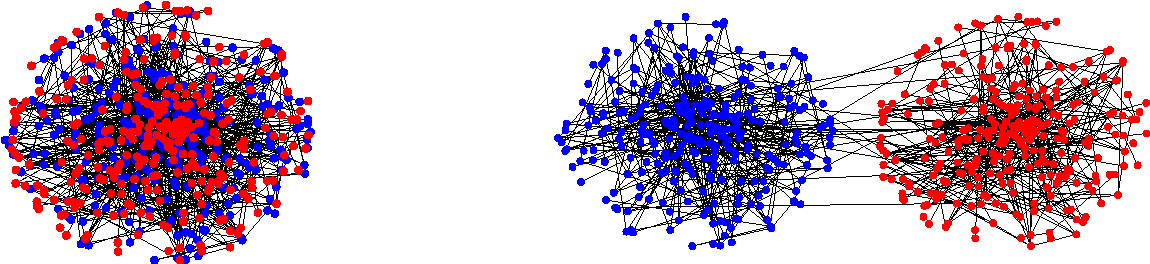
\includegraphics[width=0.7\textwidth]{figs/sbm2}
\pause
\vfill

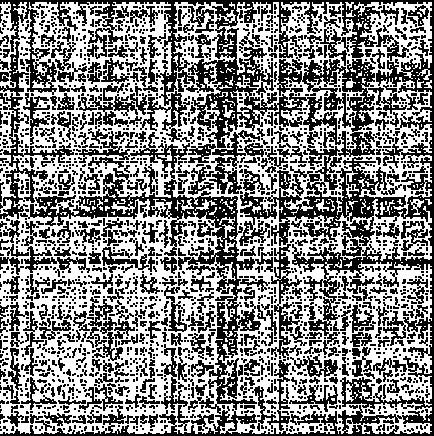
\includegraphics[width=0.25\textwidth]{figs/disorder}
\hspace{30pt}
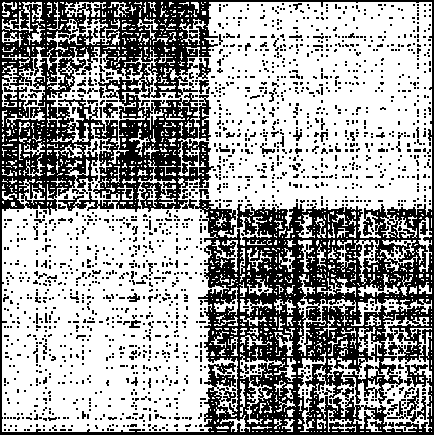
\includegraphics[width=0.25\textwidth]{figs/order}
\end{center}
\end{frame}


\begin{frame}{Clustering the stochastic block model}

$A\sim SBM(a/n, b/n, n, 2)$ sparse. \\
Statistical threshold for detection: $(a-b)^2>2(a+b)$.

\bigskip
Spectrum doesn't concentrate (high degree vertices dominate it)
Laplacian is not useful for clustering
\begin{center}
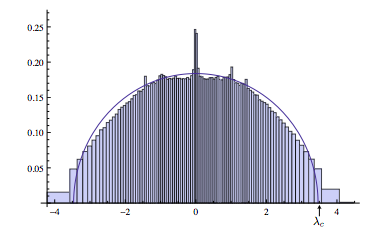
\includegraphics[height=.25\textwidth]{figs/spectral}
\end{center}

Other methods succeed. Example: semidefinite programming.
\let\thefootnote\relax\footnotetext{\tiny{Krzakala, Moore, Mossel, Neeman, Sly, Zdeborov\'a, Zhang, 2013}}
\let\thefootnote\relax\footnotetext{\tiny{Deshpande, Abbe, Montanari, 2014}}
\let\thefootnote\relax\footnotetext{\tiny{Abbe, Bandeira, Hall, 2014}}

\end{frame}

\begin{frame}{Spectral redemption}
\bigskip
Consider the non-backtracking operator (from linearized BP)
$$B_{(i\to j) (i'\to j')} = \left\{ \begin{matrix} 1 \text { if } j=i' \text{ and } j'\neq i \\ 0 \text{ otherwise}\end{matrix} \right.$$
\begin{center}

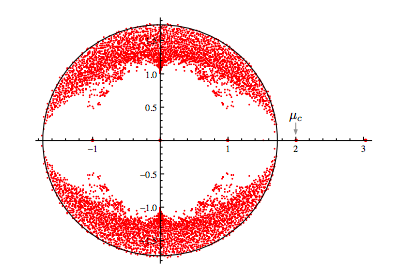
\includegraphics[height=.25\textwidth]{figs/nb}
\end{center}
Second eigenvector of $B$ reveals clustering structure
\let\thefootnote\relax\footnotetext{\tiny{Krzakala, Moore, Mossel, Neeman, Sly, Zdeborov\'a, Zhang, 2013}}
\let\thefootnote\relax\footnotetext{\tiny{Bordenave, Lelarge, Massoulie,  2015}}



\end{frame}

\begin{frame}{Bethe Hessian}

$$BH(r) = (r^2 -1 )I - rA + D$$
\smallskip

Fixed points of BP $\longleftrightarrow$ Stationary points of Bethe free energy

\smallskip
Second eigenvector reveals clustering structure


Pitfall: highly dependent in the model. % sensitive to model misspecification.

\begin{minipage}{0.48\textwidth}
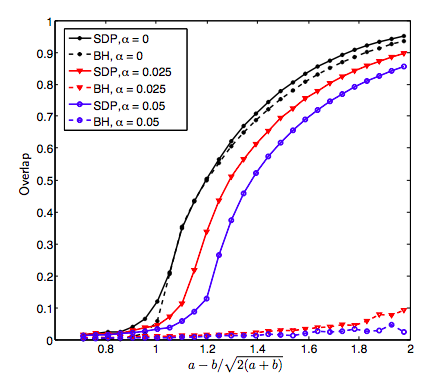
\includegraphics[width=\textwidth]{figs/plot}
\end{minipage}
\begin{minipage}{0.49\textwidth}
\pause
{\small
\textbf{Goal:} Combine graph operators $I,D,A,\ldots$ to generate robust ``data-driven spectral methods" for problems in graphs
}
\end{minipage}

\let\thefootnote\relax\footnotetext{ \tiny{Saade, Krzakala, Zdeborov\'a, 2014}}
\let\thefootnote\relax\footnotetext{ \tiny{Javanmard, Montanari, Ricci-Tersenghi, 2015}}
\end{frame}


\begin{frame}{Graph neural networks}{sGNN$(\mathcal M)$}

Power method: $v^{t+1} = Mv^t \quad \quad t=1,\ldots, T$.

\pause
\smallskip
Graph with adjacency matrix $A$. Set $\mathcal M=\{I_n, D, A, A^2,\ldots, A^{2^J}\}$,
\begin{equation*}
v^{t+1}_{\visible<3->l} = \visible<5->{\color{red}\rho \color{black}} \left( \sum_{M \in \mathcal{M}}  M v^{t} \theta_{M\visible<3->{\color{red},l}}^{\color{red}\visible<4->t}  \right) ~,\, \visible<3->{l=1,\dots ,d_{t+1}} %\\
%v^{t+1}_l &=&   \sum_{M \in \mathcal{A}} {\theta}_{M,l}^{t} B x^{t} ~,\,l=\frac{d_{t+1}}{2}+1,\dots d_{t+1}  ~,\nonumber 
\end{equation*}

with $v^t\in \mathbb R^{n\times d_t}$, \\
$\Theta=\{ \theta_1^t, \dots, \theta_{|\mathcal{M}|}^{t} \}_t$, 
${\theta}_M^{t} \in \mathbb{R}^{d_t \times d_{t+1}}$ trainable parameters. 

\bigskip

\begin{itemize}
\item<6-> Extension to line graph (GNN with non-backtracking).
\item<6-> Extension to power graph $\min (1, A^t)$
\item<7-> Equivariant wrt permutations $G \mapsto \phi(G)$ then $G_\Pi \mapsto \Pi \phi(G)$.
%\item<8-> Preliminary theoretical analysis of energy landscape.
%\begin{itemize}
%\item<9-> Strong assumptions $\Rightarrow$ local minima have low energy.
%\end{itemize}
\end{itemize}

\let\thefootnote\relax\footnotetext{\tiny{Scarselli, Tsoi, Hagenbuchner, Monfardini, 2009}}
\let\thefootnote\relax\footnotetext{\tiny{Chen, Li, Bruna, 2017}}

\end{frame}

\begin{frame}{Numerical performance. SBM $k=2$}

{\small 
\begin{center}
Overlap as function of SNR
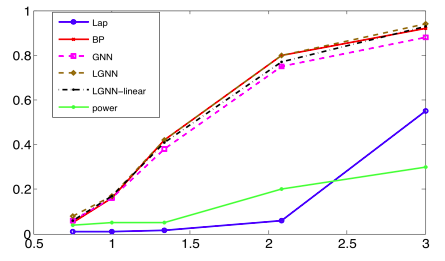
\includegraphics[width=0.7\textwidth]{figs/bruna}
\end{center}

Theoretical result: Under simplifications one can show that all local minima have small loss. 

\pause
\vfill

Extension to unsupervised setting: Max-cut on random regular graphs.

}

\let\thefootnote\relax\footnotetext{\tiny{Chen, Li, Bruna, 2017}}
\let\thefootnote\relax\footnotetext{\tiny{Yao, V., Bandeira, 2019}}
\end{frame}

\begin{frame}{Motivating example 2}{Quadratic assignment problem}
$A,B$ $n\times n$ matrices. $\Pi:$ set of $n\times n$ permutation matrices.

$$\text{Quadratic assignment}: \max_{X\in \Pi} \operatorname{Trace}(AXBX^\top)$$
\smallskip

\pause
It includes many relevant problem as particular cases:
\begin{itemize}
\item Graph matching: {\scriptsize $\min_{X\in \Pi} \|AX-XB\|_F^2$\pause$=\|AX\|^2+\|XB\|^2 - 2 \langle AX, XB \rangle$} %\operatorname{Trace}(AXB^\top X^\top)$}.
\includegraphics[height=.2\textwidth]{figs/matching}
\item<4-> Graph isomorphism
\end{itemize}
\color{white}

 Graph isomorphism.

Traveling salesman problem.

Gromov-Hausdorff distance of finite metric spaces.

%\begin{tikzpicture}[remember picture,overlay]
%    \node[xshift=-2cm,yshift=-8cm] at (current page.north east) {\includegraphics[width=1.7cm]{tsp.png}};
%\end{tikzpicture}

%\bigskip
%It is NP-hard, even to approximate it.
\end{frame}

\begin{frame}{Motivating example 2}{Quadratic assignment problem}
$A,B$ $n\times n$ matrices. $\Pi:$ set of $n\times n$ permutation matrices.

$$\text{Quadratic assignment}: \max_{X\in \Pi} \operatorname{Trace}(AXBX^\top)$$
\smallskip

It includes many relevant problem as particular cases:
\begin{itemize}
\item Graph matching: $\min_{X\in \Pi} \|AX-XB\|_F^2$.
\item Graph isomorphism.
\item Traveling salesman problem.
\end{itemize}
\begin{center}
\includegraphics[height=.17\textwidth]{figs/tsp.png} \end{center}


\color{white}

Gromov-Hausdorff distance of finite metric spaces.
%\bigskip
%It is NP-hard, even to approximate it.
\end{frame}

\begin{frame}{Motivating example 2}{Quadratic assignment problem}
$A,B$ $n\times n$ matrices. $\Pi:$ set of $n\times n$ permutation matrices.

$$\text{Quadratic assignment}: \max_{X\in \Pi} \operatorname{Trace}(AXBX^\top)$$
\smallskip

It includes many relevant problem as particular cases:
\begin{itemize}
\item Graph matching: $\min_{X\in \Pi} \|AX-XB\|_F^2$.
\item Graph isomorphism.
\item Traveling salesman problem.
\item Gromov-Hausdorff distance of finite metric spaces.
\end{itemize}

\vspace{0.09\textwidth}

It is NP-hard, even to approximate it.
\vspace{0.1\textwidth}
\end{frame}


\begin{frame}{GNN approach to quadratic assignment}

%Graph matching: {\scriptsize $\min_{X\in \Pi} \|G_1 X-XG_2\|_F^2$\pause$=\|G_1X\|^2+\|XG_2\|^2 - 2 \langle G_1X, XG_2 \rangle$} %\operatorname{Trace}(AXB^\top X^\top)$}.
%\begin{center}
%\includegraphics[height=.2\textwidth]{matching}
%\end{center}
%\vspace{-.5 cm}

Siamese neural network:

\begin{center}
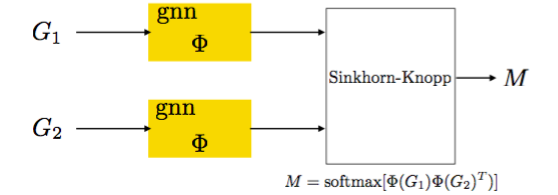
\includegraphics[height=.2\textwidth]{figs/gnn_qap}
\end{center}

$G_2 = \pi \star G_1 \oplus N \quad\quad N\sim $ i.i.d. bit flip 

$G_1\sim$ Erdos-Renyi

$G_1\sim$ Random regular

\let\thefootnote\relax\footnotetext{\tiny{Nowak, V., Bandeira, Bruna, 2017}}
\end{frame}

\begin{frame}{Numerical experiments}
\begin{center}
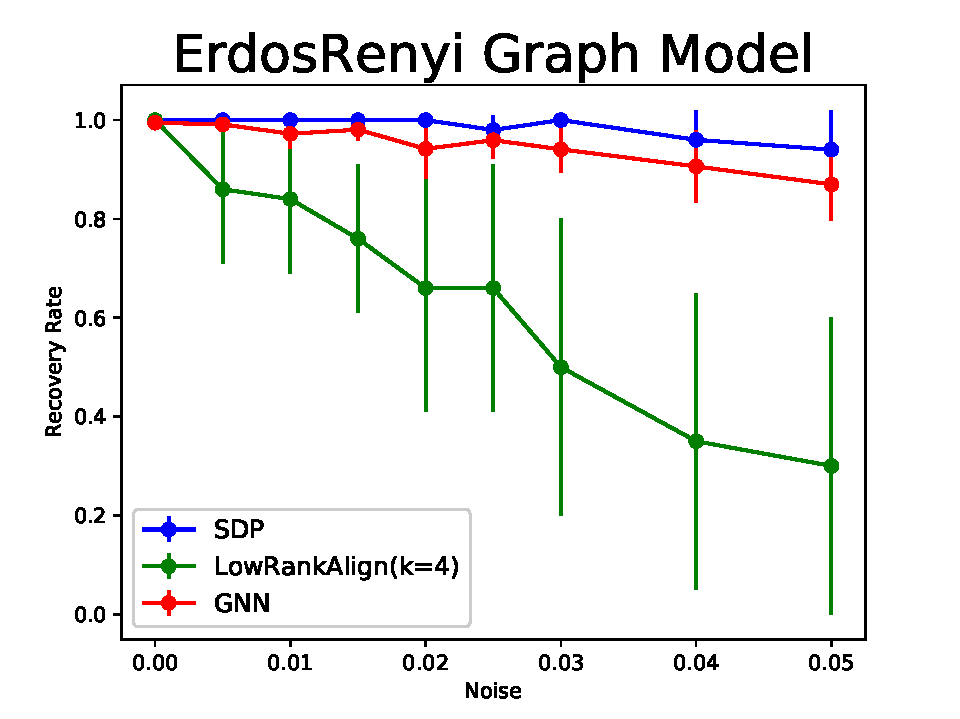
\includegraphics[width=.45\textwidth]{figs/ErdosRenyi}
\includegraphics[width=.45\textwidth]{figs/regular}
\end{center}

%{\small GNN runs in $O(n^2)$ , LowRankAlign is $O(n^3)$, SDP in $O(n^4)$.}
\pause
\vfill
\begin{center}
\begin{tabular}{cc}
	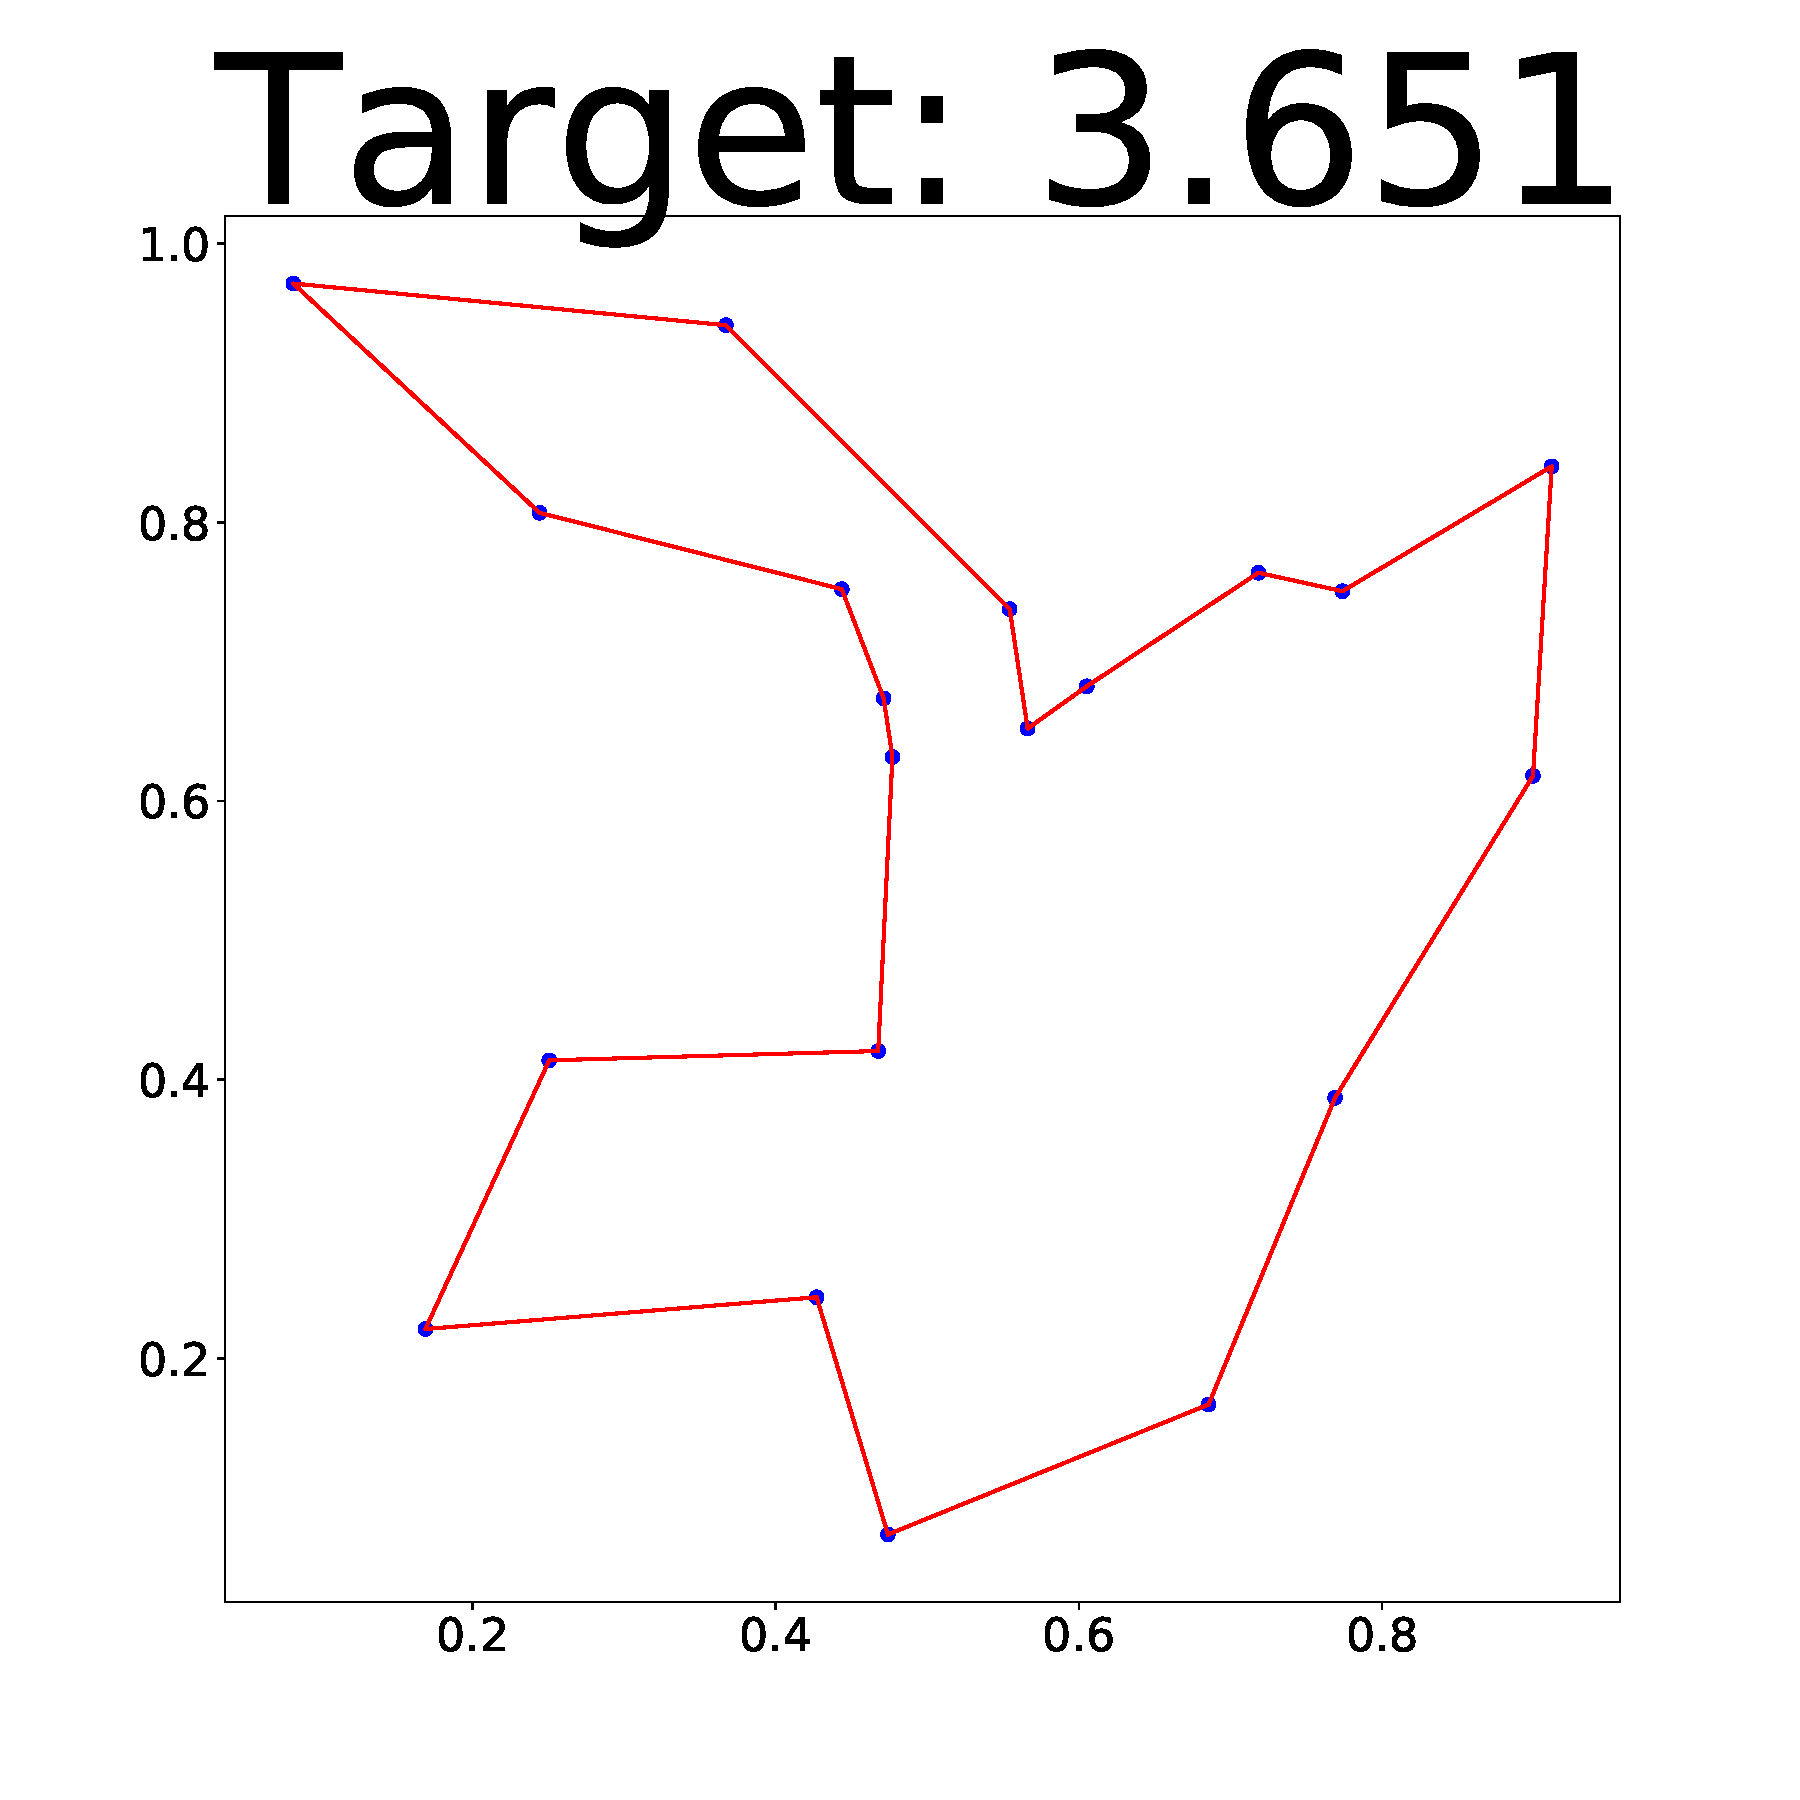
\includegraphics[width=0.15\textwidth]{figs/ground_tsp4.pdf} &
	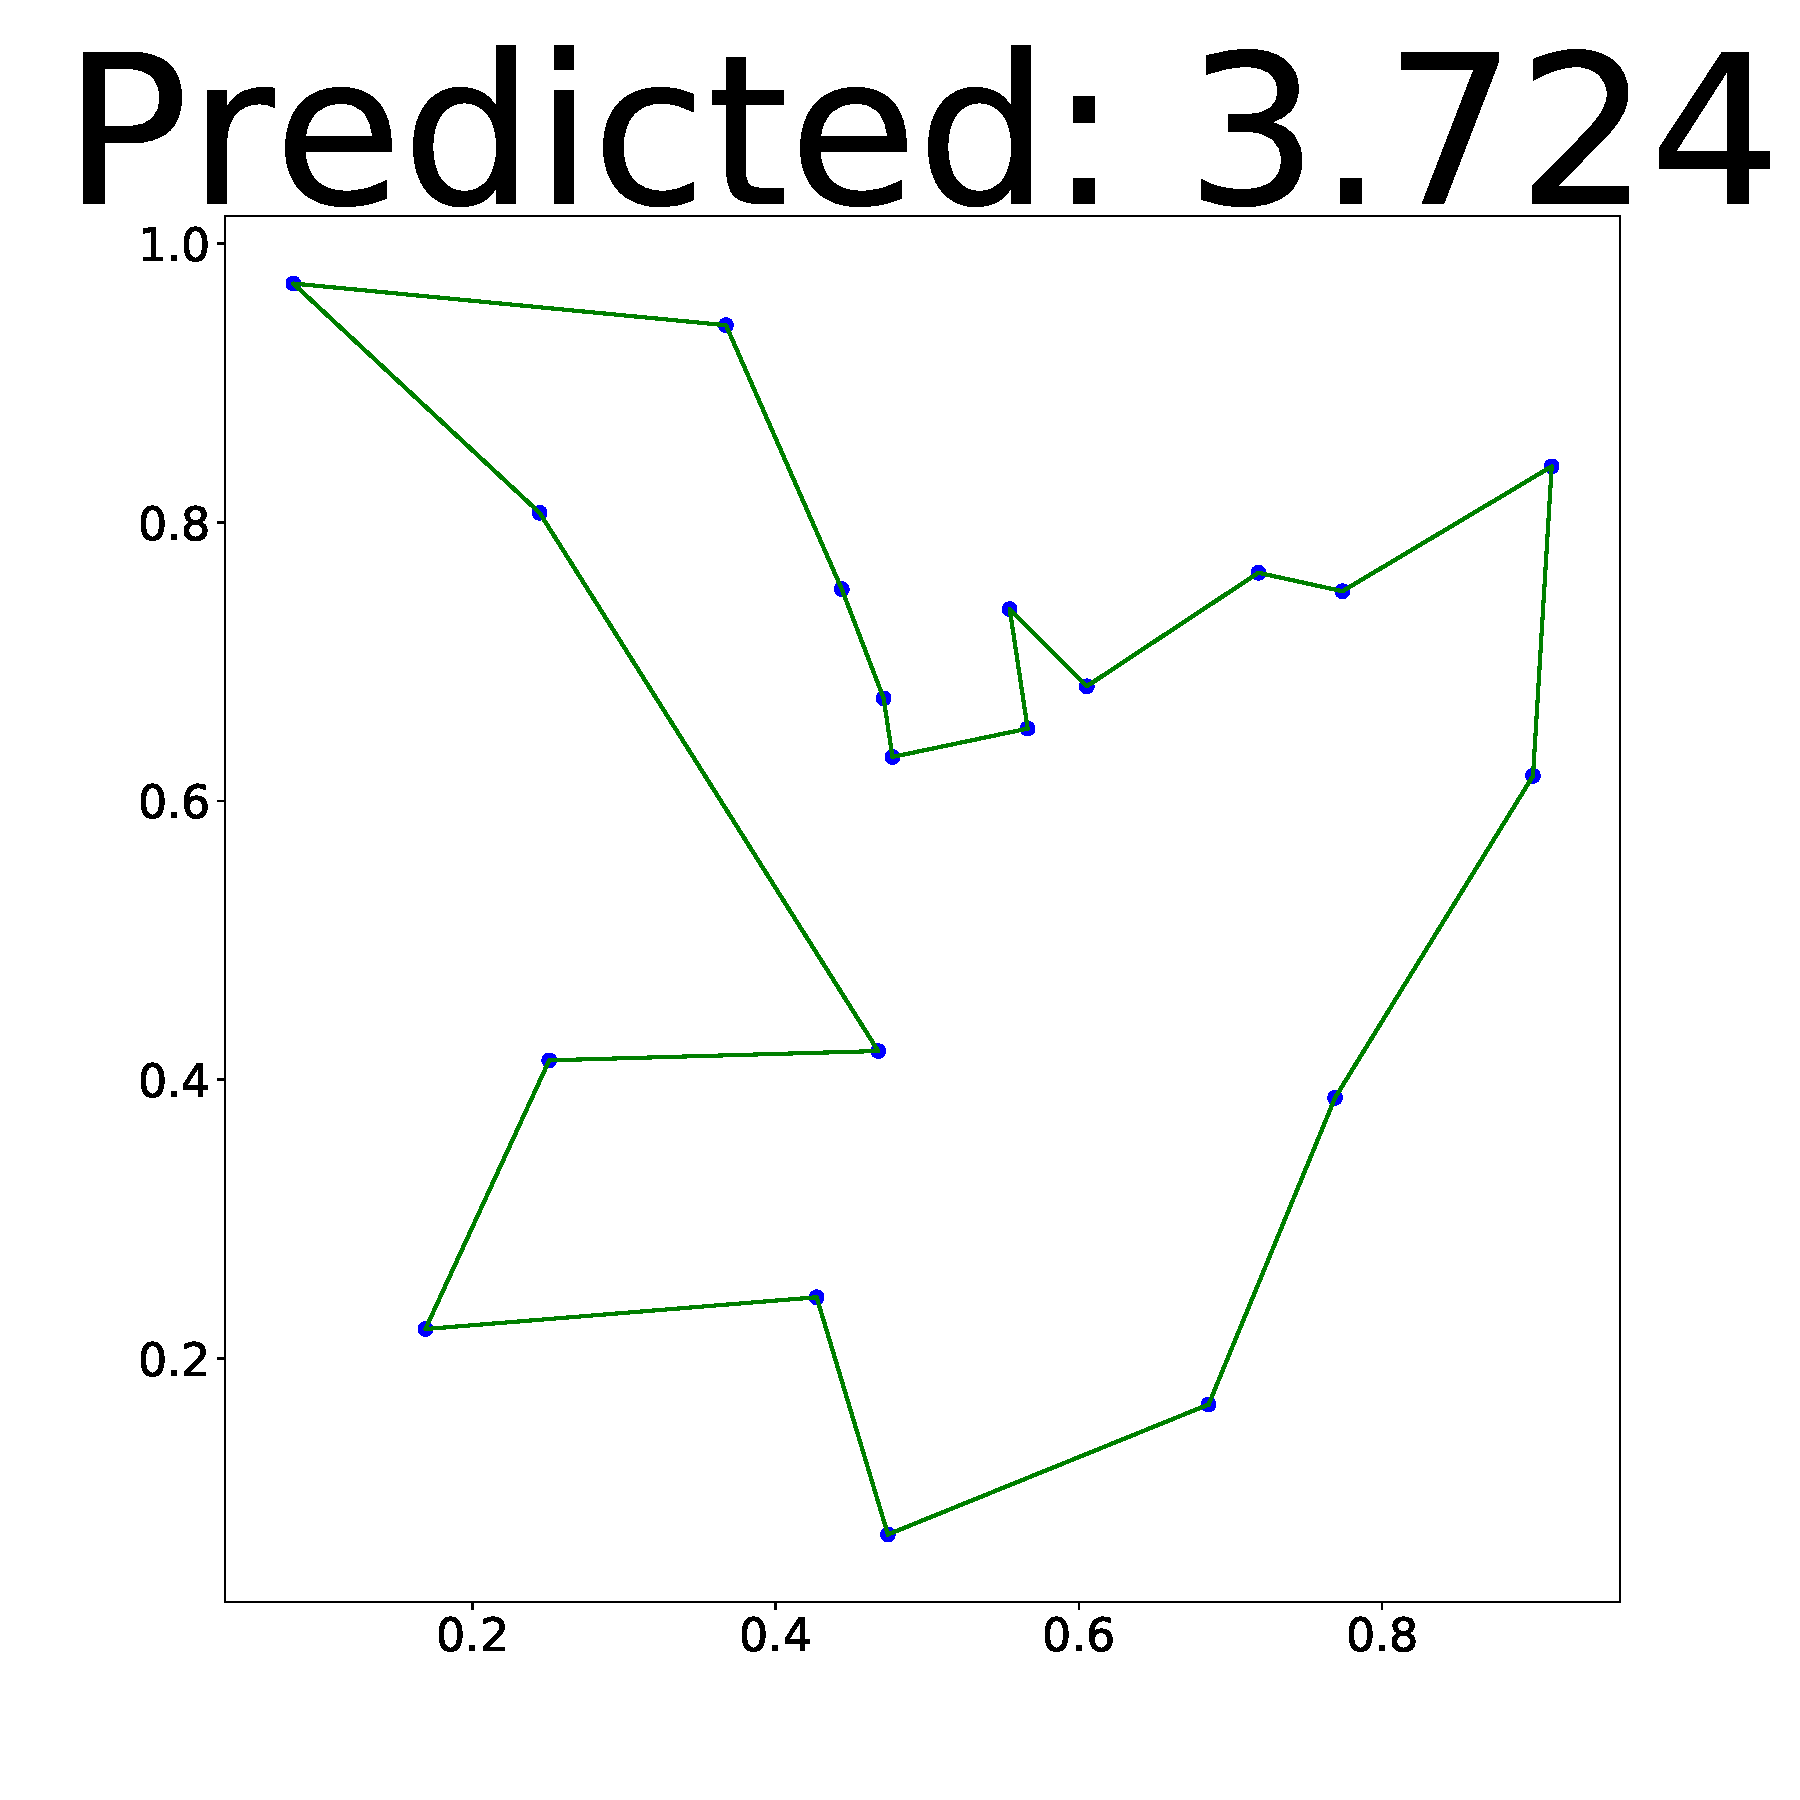
\includegraphics[width=0.15\textwidth]{figs/pred_tsp4.pdf} \\
	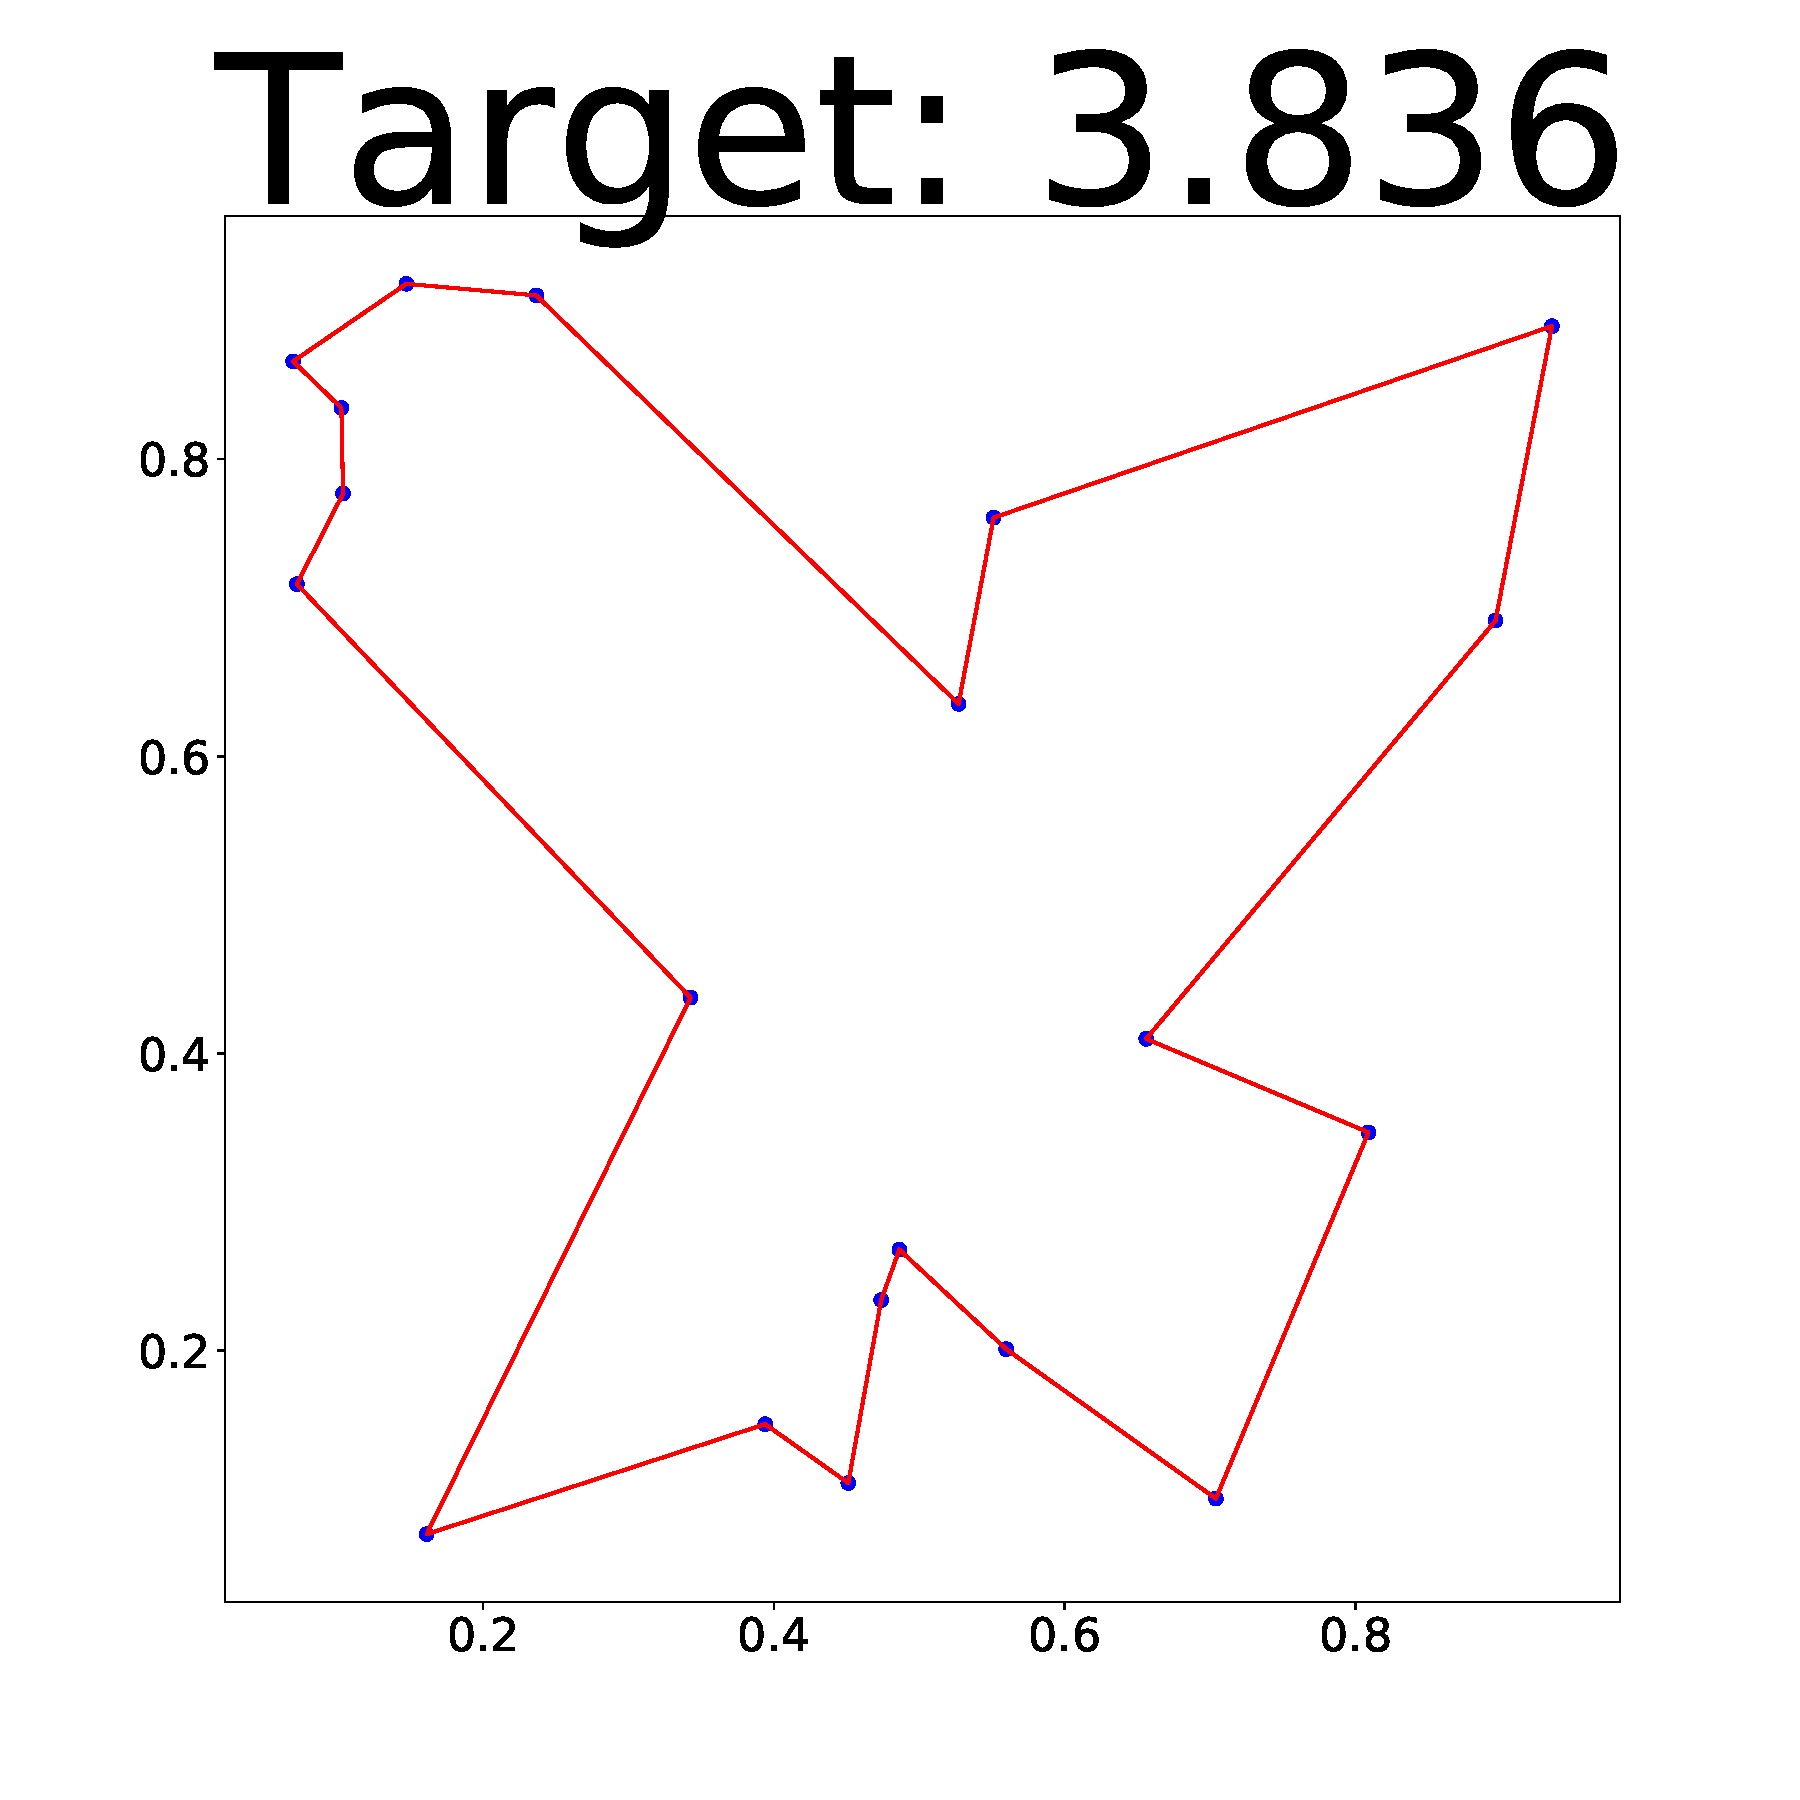
\includegraphics[width=0.15\textwidth]{figs/ground_tsp0.pdf} &
	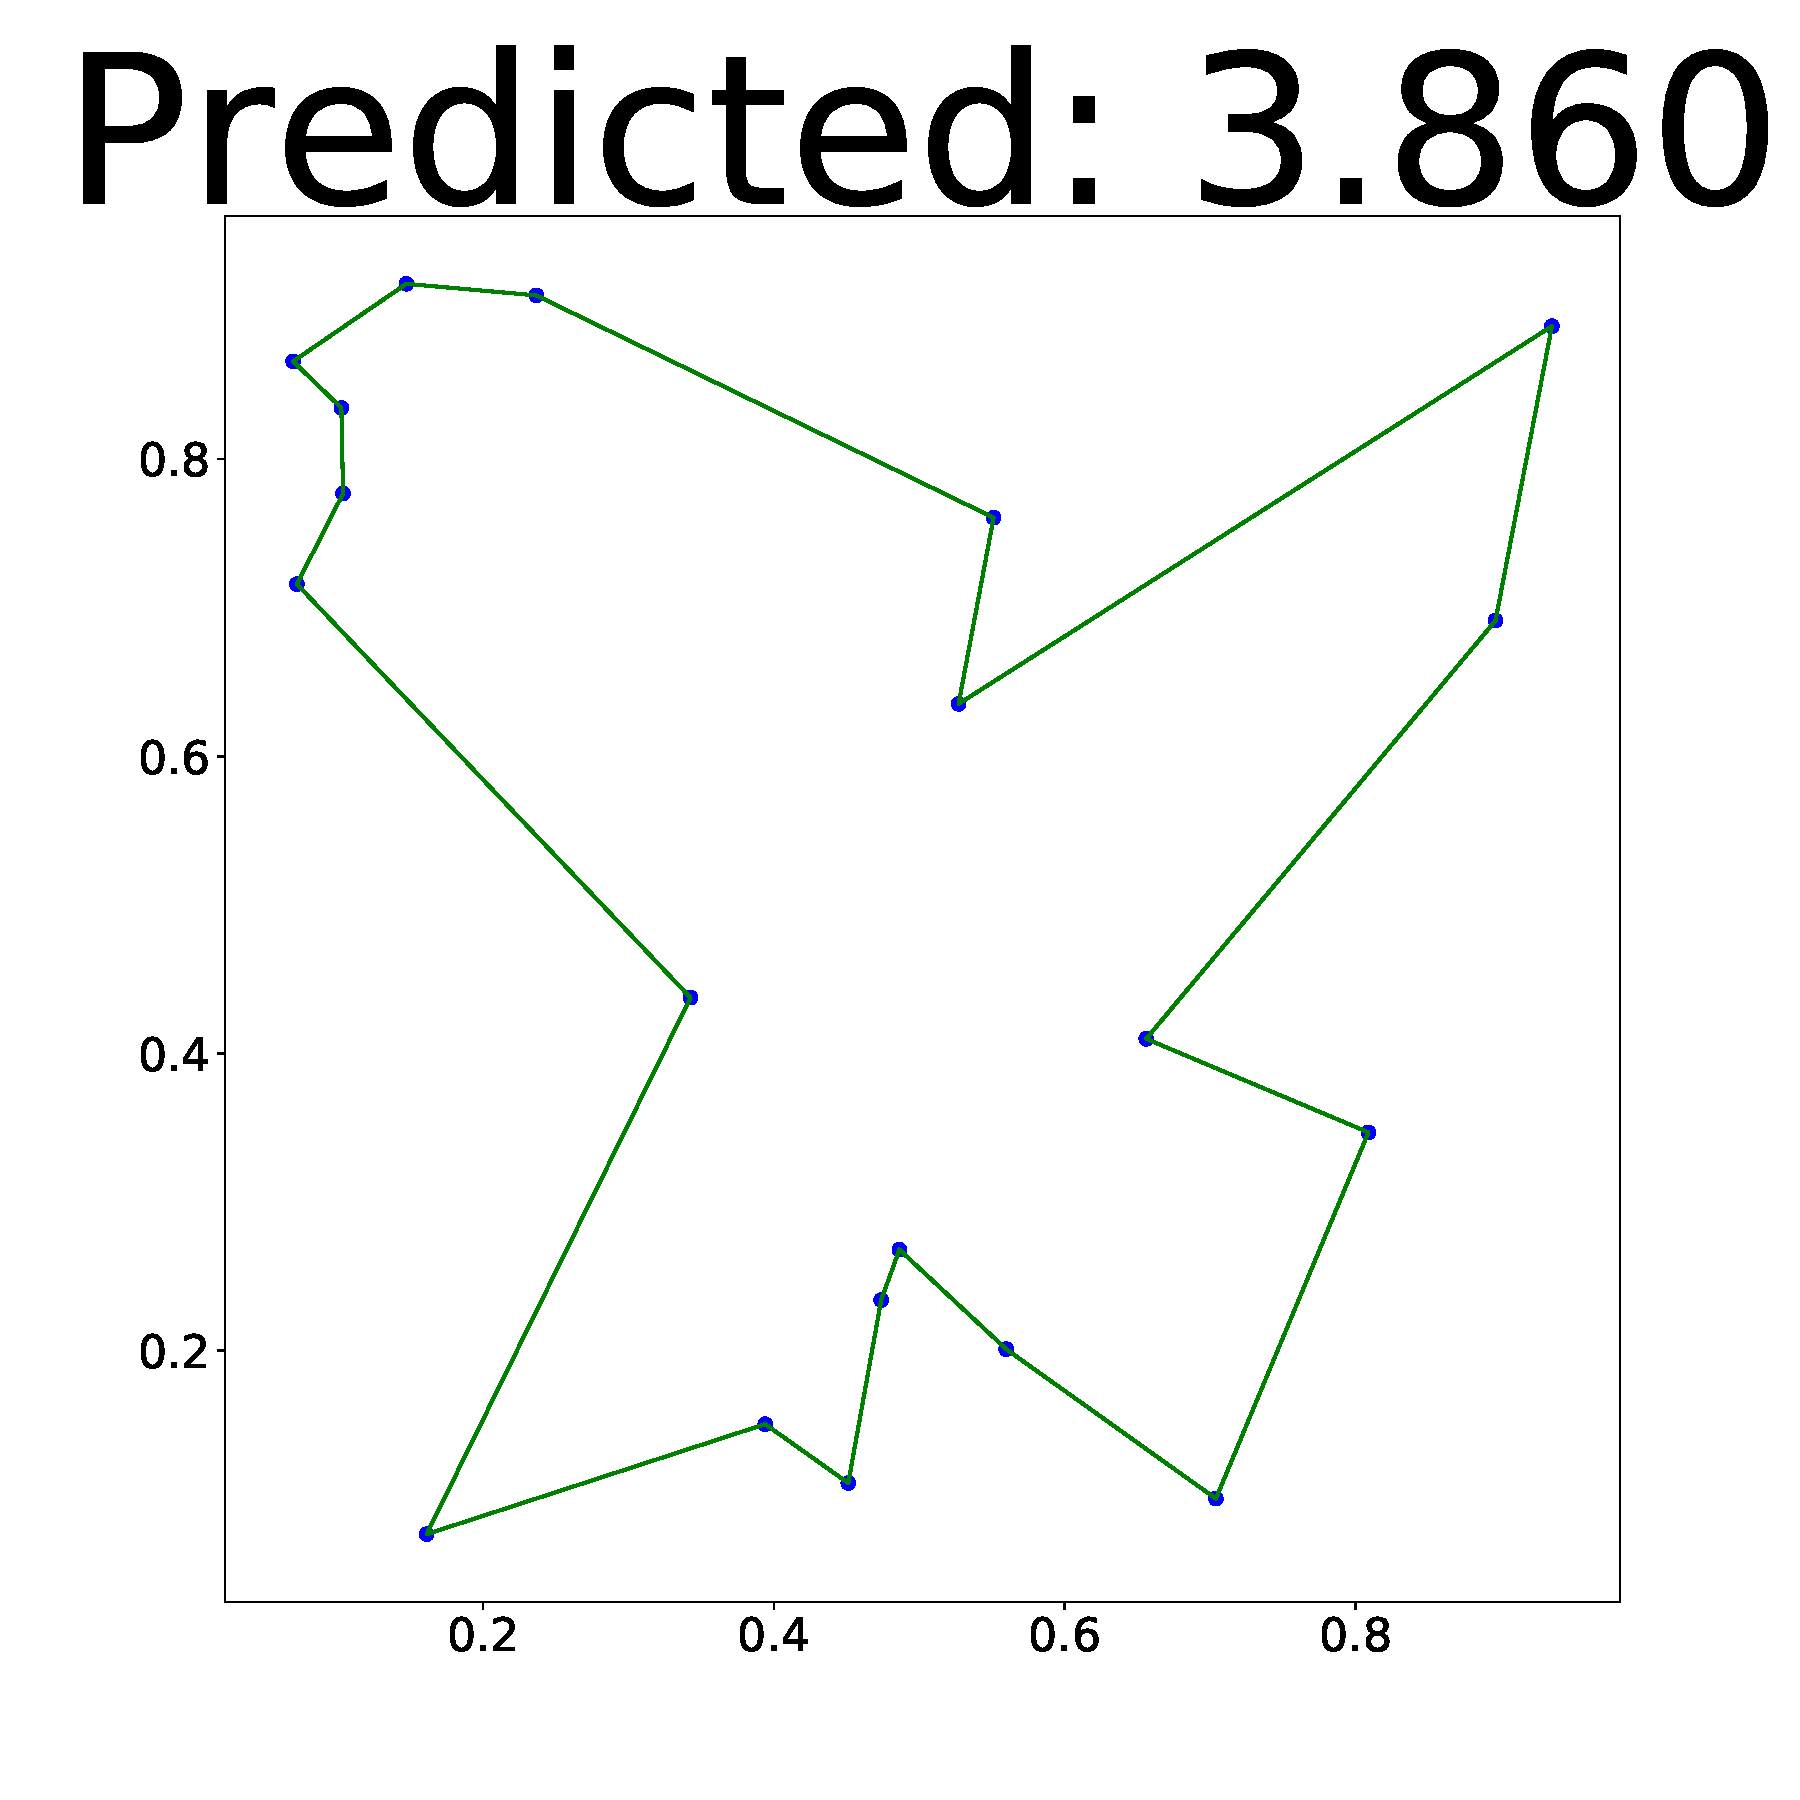
\includegraphics[width=0.15\textwidth]{figs/pred_tsp0.pdf} 
\end{tabular}	
\end{center}
\let\thefootnote\relax\footnotetext{\tiny{Nowak, V., Bandeira, Bruna, 2017}}
\end{frame}

\begin{frame}{Other GNN formulation}{Message passing neural network}
$$a^{(k)}_v=\text{AGGREGATE}^{(k)}\left(\{h_u^{(k-1)}: u\in \mathcal N(u)\} \right)$$
$$h^{(k)}_v=\text{COMBINE}^{(k)}\left( h_v^{(k-1)}, a_v^{(k)} \right)
$$
\pause
\begin{itemize}
\item There exist many formulations of GNN
\item All satisfy one essential property: 
\begin{itemize}
\item invariance or equivariance with respect to permutations
\item node labels are not intrinsic
\end{itemize}
\end{itemize}


\let\thefootnote\relax\footnotetext{\tiny{Hamilton, Ying, Leskovec, 2017}}

\end{frame}

\begin{frame}{How powerful are graph neural networks?}

Q: How good are they at distinguishing non-isomorphic graphs?
\pause
\bigskip

A: MPNN can be as powerful as the Weisfeler-Lehman test (1968).
\\
W-L test is as powerful as the LP relaxation (Ullman et al 1994). 

\pause
\bigskip

In particular MPNN cannot distinguish between non-isomorphic regular graphs with the same degree. 
\begin{center}
    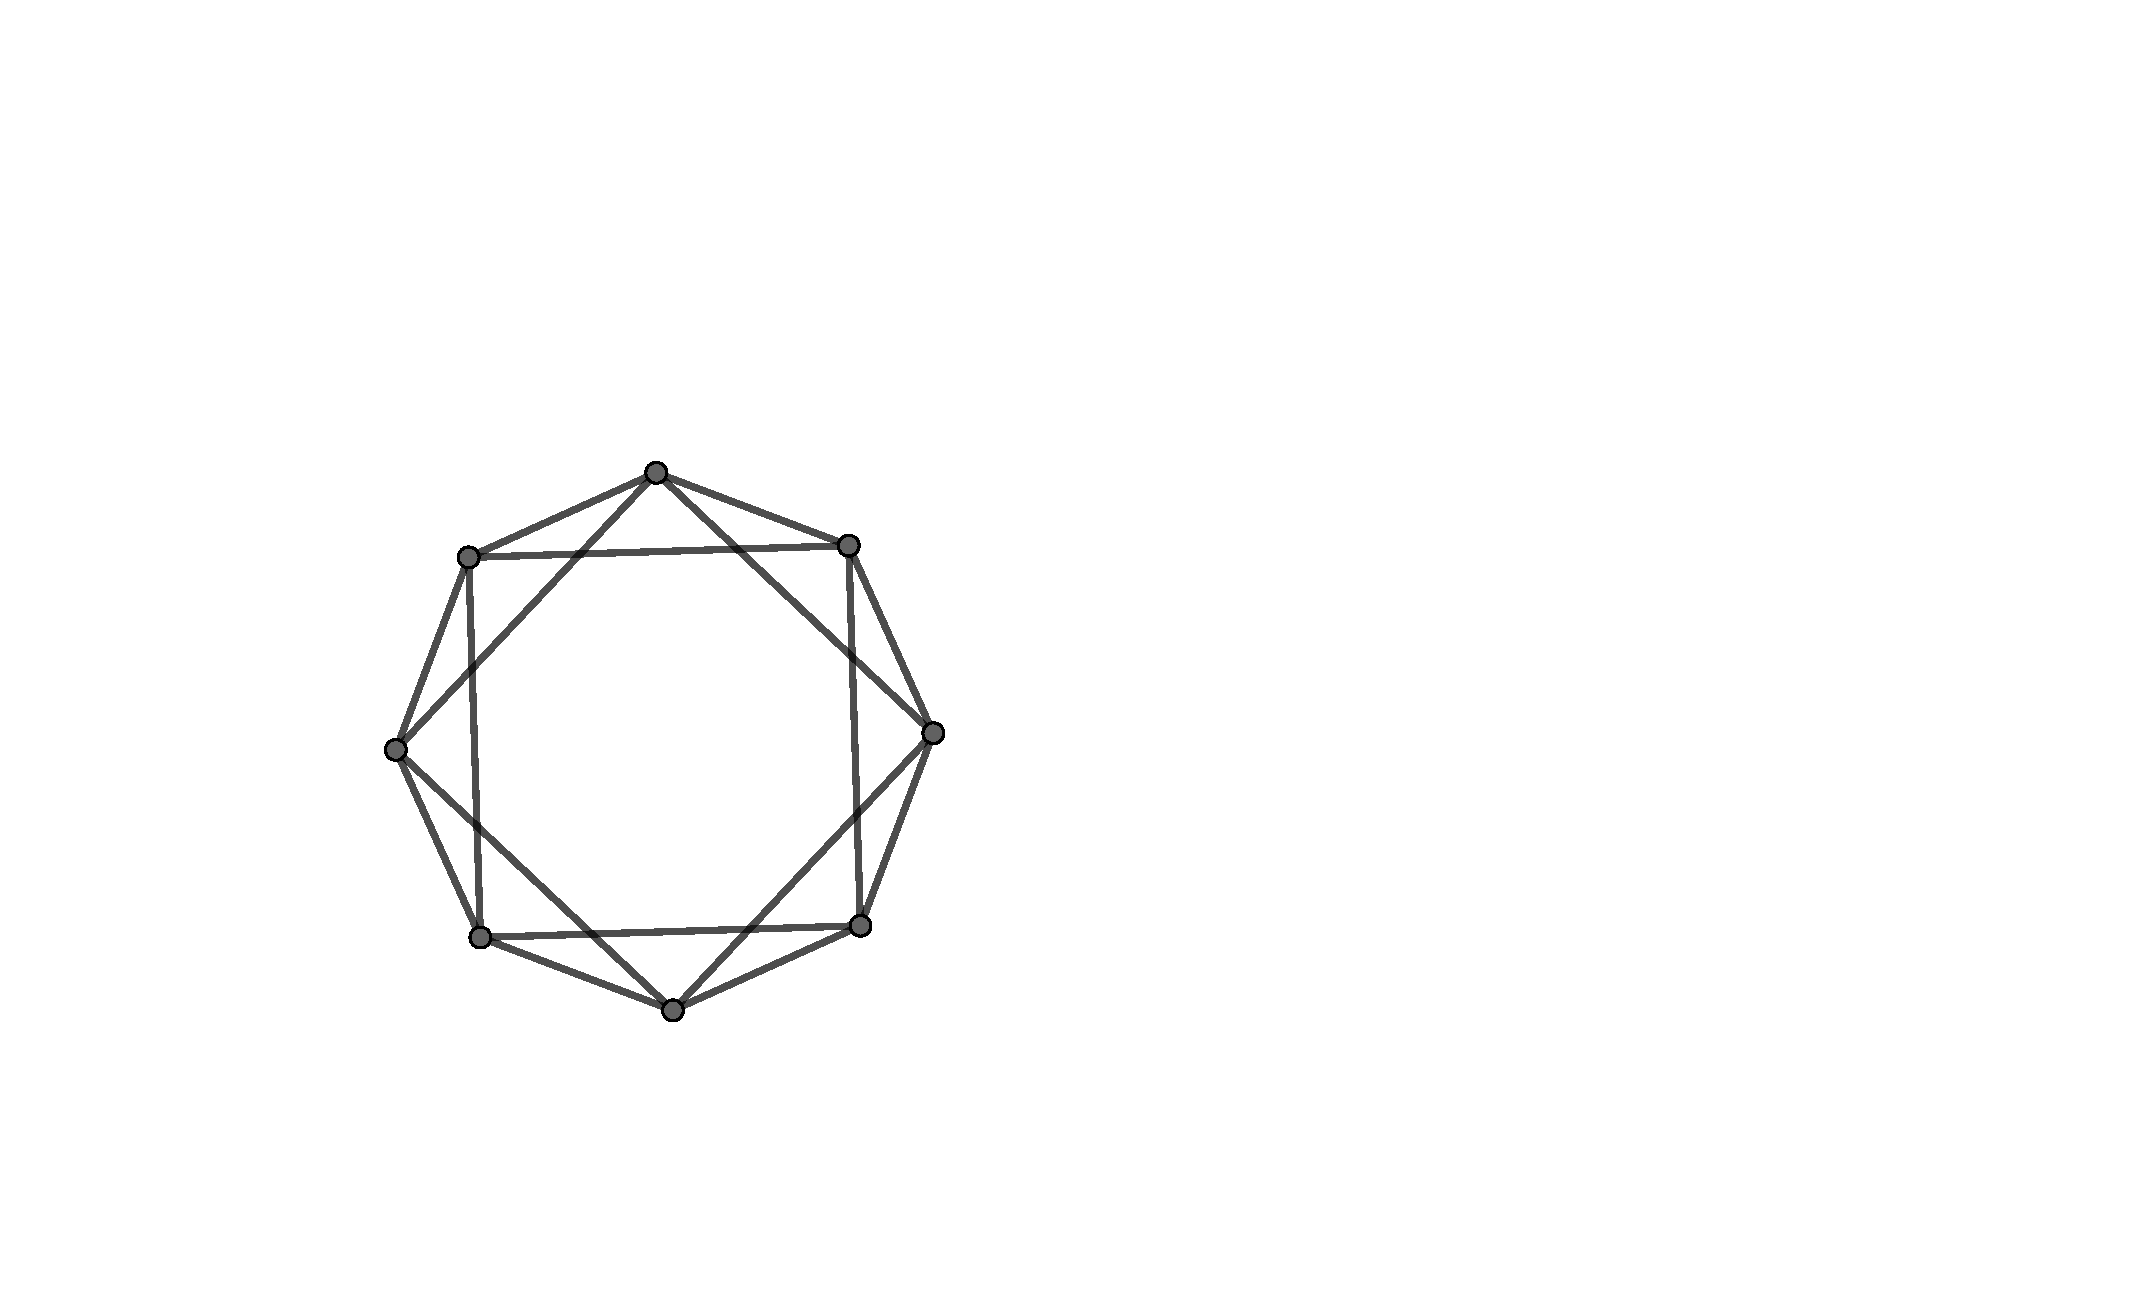
\includegraphics[width=0.15\textwidth,trim={6cm 4.8cm 20cm 7.8cm},clip]{figs/skl2black}
    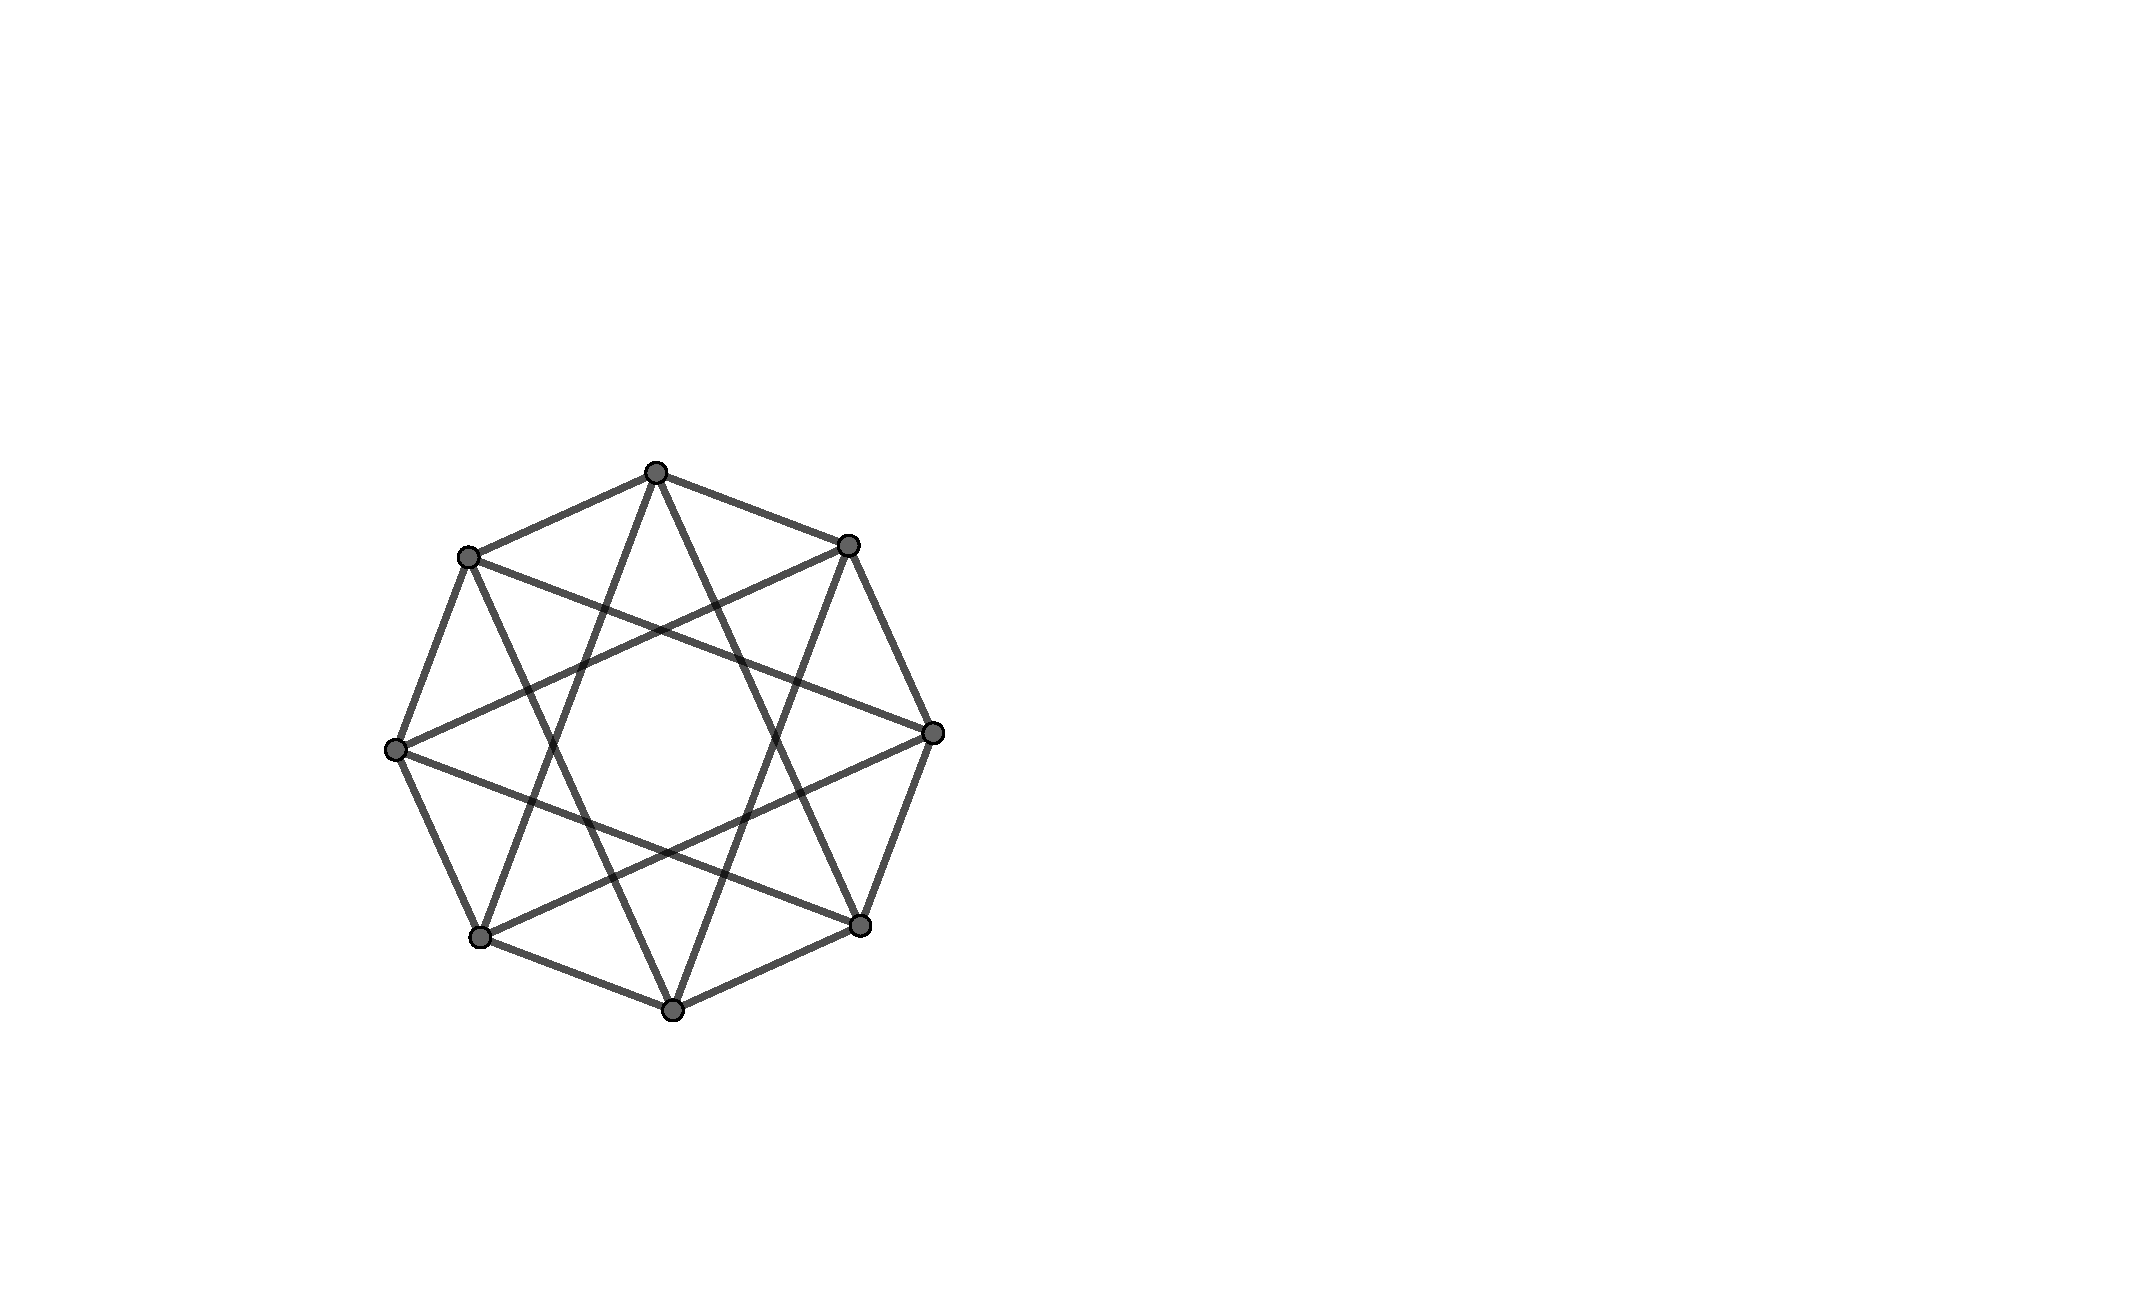
\includegraphics[width=0.15\textwidth,trim={6cm 4.8cm 20cm 7.8cm},clip]{figs/skl3black}
\end{center}
 
\let\thefootnote\relax\footnotetext{\tiny{Xu, Hu, Leskovec, Jekelga 2019}}
\end{frame}

\begin{frame}{Invariant functions on graphs}
%Let $T^k \in \mathbb R^{n^k}$ $k$-tensor, with the symmetric group $S_n$ acting in each dimension (with the same element). 

\begin{itemize}
\item Linear case:
\begin{itemize}
\item If $L: \mathbb R^{n^k} \to \mathbb R$ invariant, then
$vec(L) = \pi^{\otimes k} vec(L)$.
\item If $ L:  \mathbb R^{n^k} \to \mathbb R^{n^k}$ equivariant, then
$vec(L) = \pi^{\otimes 2k} vec(L)$
\bigskip
\item The space of invariant [equivariant] linear functions on $k$-tensors has dimension $b(k)$ [$b(2k)$]. \\ {\scriptsize ($b(k)$ denotes Bell Number: number of partitions of a size k set).}
\pause
\end{itemize}
\vfill
\item Universal approximation:
\begin{itemize}
\item Invariant networks constructed by composition of linear invariant  layers $L_t:\mathbb R^{n^k\times a} \to \mathbb R^b$ with ReLU or sigmoid activation functions universally approximate the space of invariant functions.
{\scriptsize \item Extension to equivariant functions.}
\pause
\smallskip
\\ Arbitrary high order tensors are needed. 
\smallskip
\\ Rates of convergence are not known. 
\end{itemize}
\end{itemize}
\let\thefootnote\relax\footnotetext{\tiny{Maron, Ben-Hamu, Shamir, Lipman, 2019}}
\let\thefootnote\relax\footnotetext{\tiny{Maron, Fetaya, Segol, Lipman, 2019}}
\let\thefootnote\relax\footnotetext{\tiny{Keriven, Peyr\'e, 2019}}
\end{frame}


\begin{frame}{Graph isomorphism equivalence to universal approximation}


\begin{block}{GIso-discriminating class of functions}
A class $\mathcal{C}$ of permutation-invariant functions from $\mathcal{X}^{n \times n}$ to $\mathbb{R}$ so that for all pairs  $G_1 \not \simeq G_2 \in \mathcal X^{n\times n}$,  there exists $ h \in \mathcal{C}$ such that $h(G_1) \neq h(G_2)$. 
\end{block}

\begin{center}
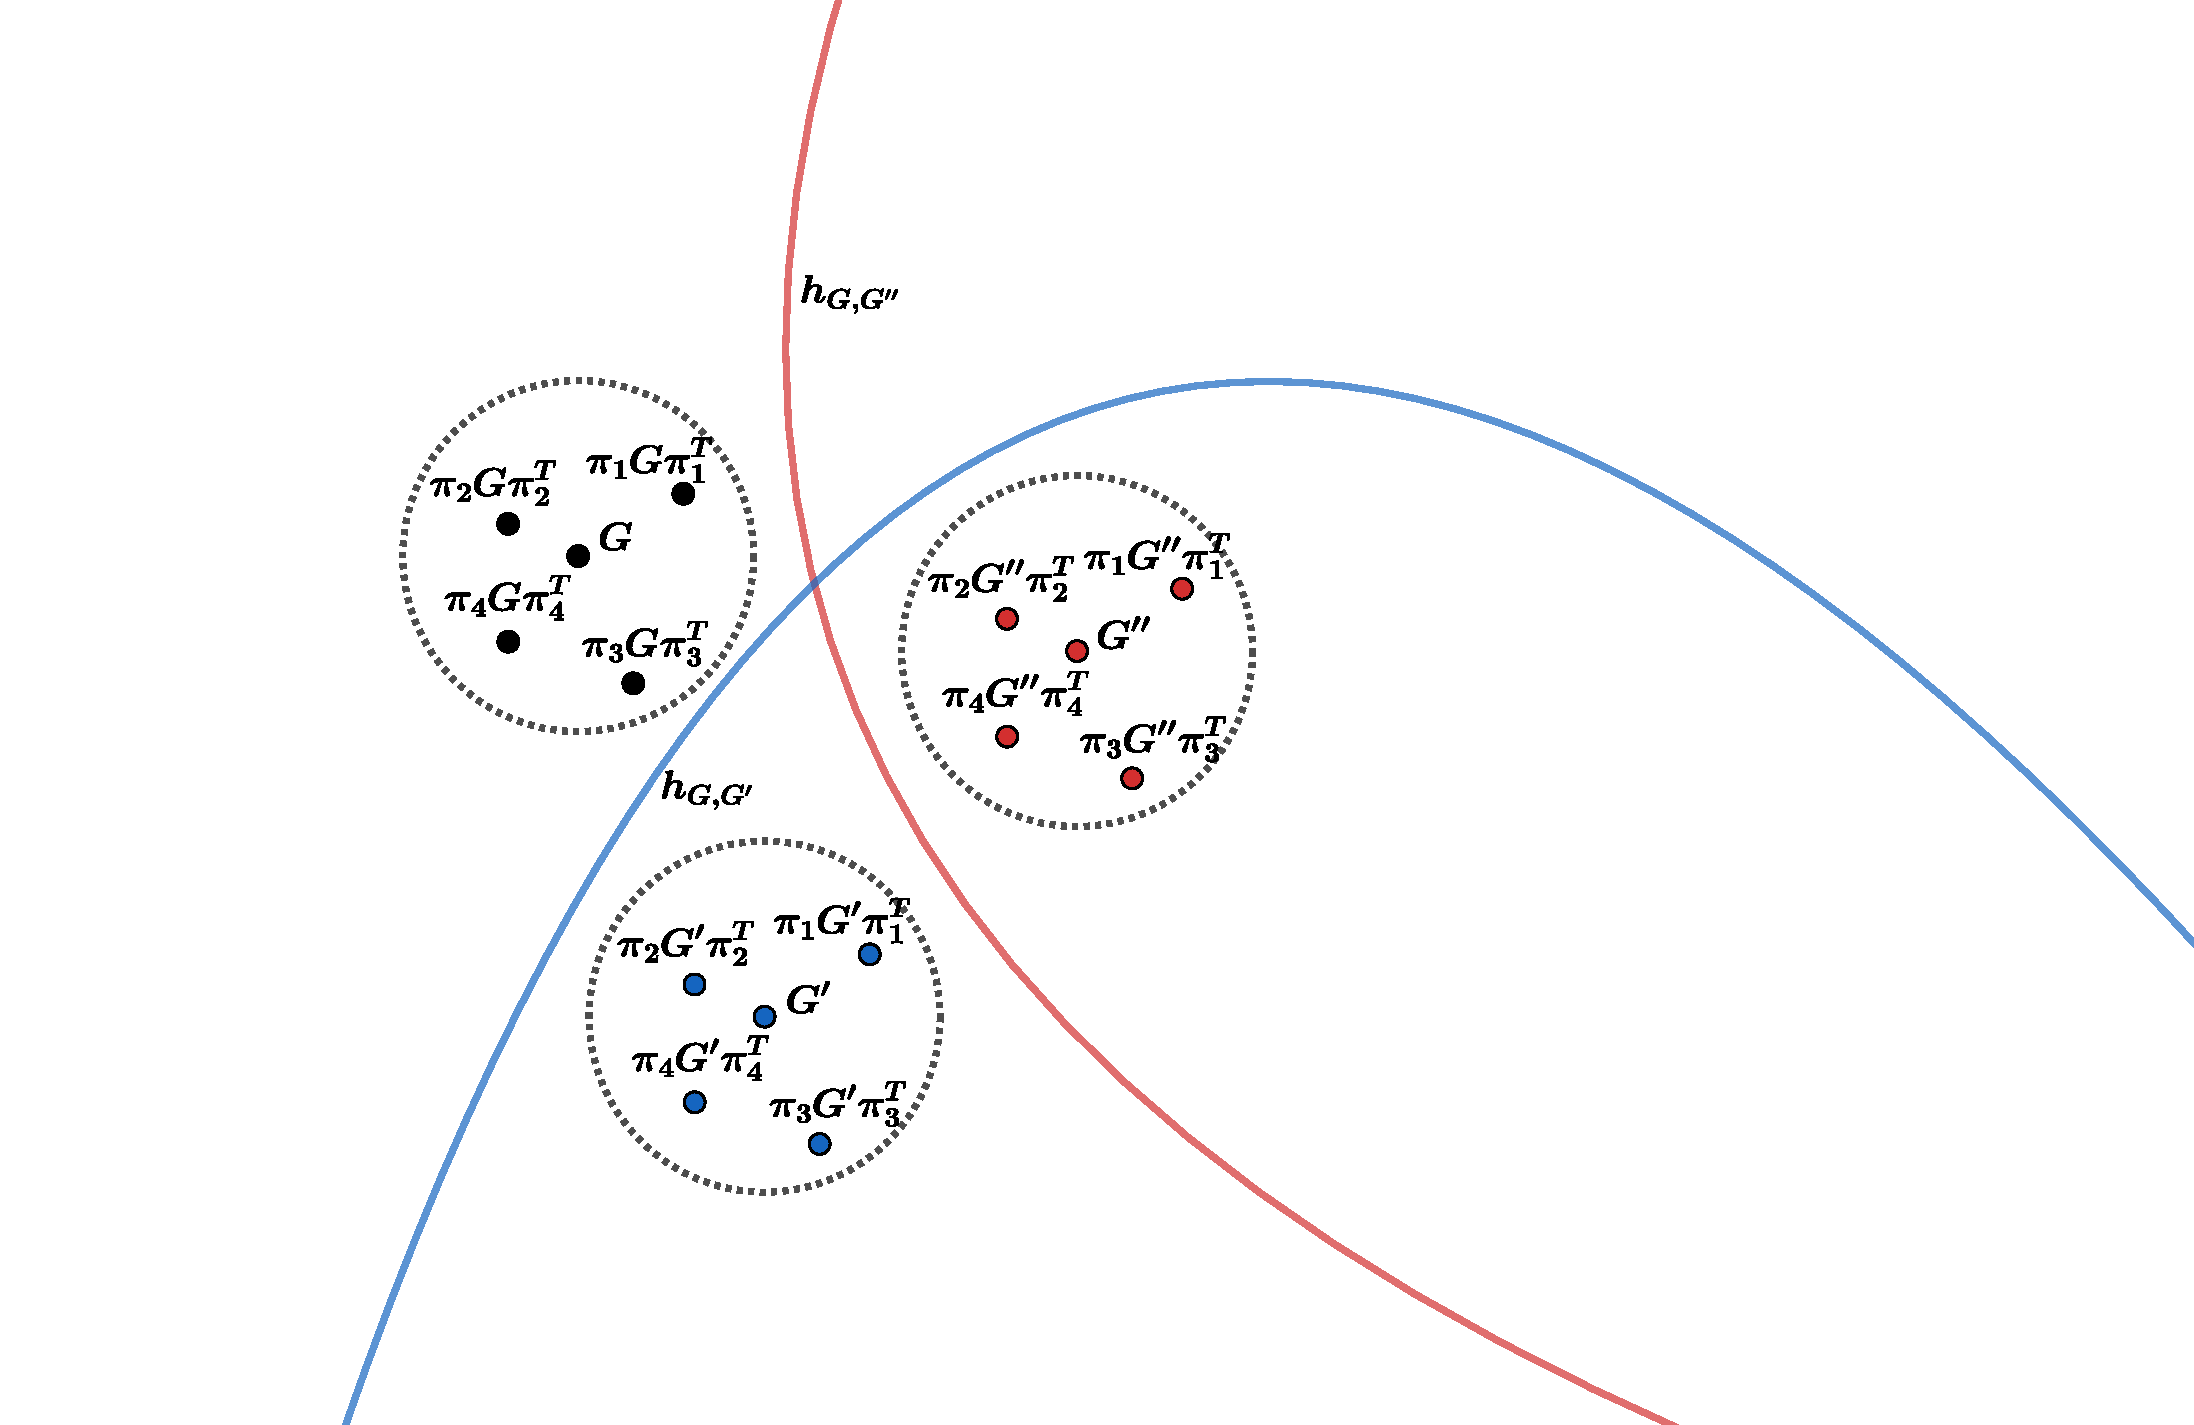
\includegraphics[width=0.4\textwidth,trim={6cm 3cm 14cm 4cm},clip]{figs/separating_functions_.pdf}
\end{center}
\let\thefootnote\relax\footnotetext{\tiny{Chen, V., Chen, Bruna, 2019}}
\end{frame}

\begin{frame}{Graph isomorphism equivalence to universal approximation}
\begin{block}{Universally approximating}
A class $\mathcal{C}$ of permutation-invariant functions from $\mathcal{X}^{n \times n}$ to $\mathbb{R}$ so that for all permutation-invariant function $f$ from $\mathcal{X}^{n \times n}$ to $\mathbb{R}$, and for all $\epsilon > 0$, there exists $h_{f,\epsilon} \in \mathcal{C}$ such that $\| f - h_{f,\epsilon} \|_{\infty} := \sup_{G \in \mathcal X^{n\times n}} |f(G) - h_{f,\epsilon}(G)| < \epsilon$
\end{block}

\bigskip

\begin{block}{Remark}
Universally approximating classes of functions are also GIso-discriminating.
\end{block}
\let\thefootnote\relax\footnotetext{\tiny{Chen, V., Chen, Bruna, 2019}}
\end{frame}

\begin{frame}{Graph isomorphism equivalence to universal approximation}

\begin{block}{$\mathcal C^{+L}$}
If $\mathcal{C}$ is a collection of functions from $\mathcal{X}^{n \times n}$ to $\mathbb{R}$, consider the set of functions from graphs $G$ to $\mathcal{NN}([h_1(G), ..., h_d(G)])$ for some finite $d$ and $h_1, ..., h_d \in \mathcal{C}$, where $\mathcal{NN}$ is a feed-forward neural network with ReLU and $L$ layers.
\end{block}

\bigskip

\begin{block}{Theorem}
If $\mathcal{C}$ is GIso-discriminating $\mathcal C^{+2}$ is universally approximating.
\end{block}
\let\thefootnote\relax\footnotetext{\tiny{Chen, V., Chen, Bruna, 2019}}
\end{frame}

\begin{frame}{Comparison of classes of functions through GIso}

$\mathcal C \subseteq \mathcal C'$ if for all pairs of non-isomorphic graphs $G_1, G_2$, if there exists $h \in \mathcal C$ so that $h(G_1)\neq h(G_2)$ then there exists $h' \in \mathcal C'$ so that $h'(G_1)\neq h'(G_2)$.
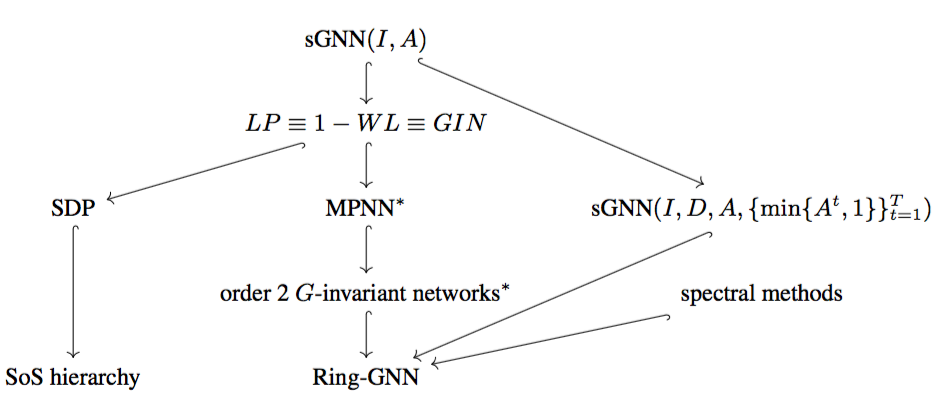
\includegraphics[width=\textwidth]{figs/GISO}

\end{frame}

\begin{frame}{Ring GNN}

{\small
Input: Graph with $n$ nodes and $d$ features: $A\in \mathbb R^{n\times n\times d}$.
% For simplicity let us assume that the output signal also has $d$ channels.
\smallskip
%All linear equivariant layers from $\mathbb{R}^{n \times n}$ to $\mathbb{R}^{n \times n}$ can be expressed as $L_\theta(A)=\sum_{i=1}^{15} \theta_i L_i(A) + \sum_{i=16}^{17} \theta_i \overline{L}_i$, where the $\{L_i\}_{i = 1, ..., 15}$.

Equivariant linear layer from $\mathbb{R}^{n \times n \times d}$ to $\mathbb{R}^{n \times n \times d'}$. For  $\theta \in \mathbb{R}^{d \times d' \times 17}$: $L_{\theta}(A)_{\cdot, \cdot, k'} = \sum_{k=1}^d \sum_{i=1}^{15} \theta_{k, k', i} L_i(A_{\cdot, \cdot, i}) + \sum_{i=16}^{17} \theta_{k, k', i} \overline{L}_i$.

Set $A^{(0)}=A$. 
\begin{eqnarray*}
B_1^{(t)}&=& \rho(L_{\alpha^{(t)}}(A^{(t)})) \\
B_2^{(t)}&=& \rho(L_{\beta^{(t)}}(A^{(t)})\cdot L_{\gamma^{(t)}}(A^{(t)})) \\
A^{(t+1)}&=& k_1^{(t)} B_1^{(t)} + k_2^{(t)} B_2^{(t)}
\end{eqnarray*}
where $k_1^{(t)}, k_2^{(t)} \in \mathbb{R}$, $\alpha^{(t)}, \beta^{(t)}, \gamma^{(t)} \in \mathbb{ R}^{d^{(t)} \times {d'}^{(t)} \times 17}$ are learnable parameters. 

Scalar output: $\theta_S \sum_{i,j} A_{ij}^{(T)} + \theta_D \sum_{i,i} A_{ii}^{(T)} + \sum_{i} \theta_{i} \lambda_{i}(A^{(T)})$, where $\theta_S, \theta_D, \theta_1, \ldots, \theta_n \in \mathbb{R}$ are trainable parameters, and  $\lambda_{i}(A^{(T)})$ is the $i$-th eigenvalue of $A^{(T)}$.
}
\end{frame}

\begin{frame}{Extensions - Future work}
\begin{itemize}
\item Explicit rates: \\ {\footnotesize Connect GNN depth/architecture with classes of graphs they separate.}
\vfill
\item Optimization landscape of GNNs: \\
{\footnotesize Current analysis of optimization landscape relies in simplified models to show that all local minima are confined in low-energy configurations.}
\vfill
\item Connection with SoS: \\
{\footnotesize For some classes of ``detecting hidden structures problems" existence of degree-$d$ SoS refutations implies success of certain (typically non-explicit) spectral methods.}
\begin{itemize}
{\footnotesize
\item Can we express such class of spectral methods with GNNs.
\item Can we learn them?}
\end{itemize}

\end{itemize}
\let\thefootnote\relax\footnotetext{\tiny{Hopkins, Kothari, Potechin, Raghavendra, Schramm, Steurer, 2017}}
\end{frame}




\begin{frame}{References}


{\small 
\textcolor{darkblue}{\textbf{Supervised Community Detection with Hierarchical Graph Neural Networks}}\\
Z. Chen, L. Li, J. Bruna, ICLR 2019\\
arXiv:1705.08415
\vfill
\textcolor{darkblue}{\textbf{A note on learning algorithms for quadratic assignment with
Graph Neural Networks }}\\
 A.\ Nowak, S. Villar, A. S. Bandeira, J. Bruna, ICML Workshop (PADL) 2017 \\
arXiv:1706.07450
\vfill
\textcolor{darkblue}{\textbf{On the equivalence between graph isomorphism testing and function approximation with GNNs}}\\
 Z.\ Chen, S. Villar, L. Chen, J. Bruna, NeurIPS 2019 \\ 
arXiv:1905.12560
}


\includegraphics[height=0.19\textheight]{figs/nsf} \hfill

\includegraphics[height=0.18\textheight]{figs/eoard} \hfill

\includegraphics[height=0.19\textheight]{figs/simons}

\end{frame}





\end{document}